\section{Results and Discussion}
\label{sec:findings}

\subsection{Main Results}
\label{sec:leaderboard}

We evaluate 22 models (18 open-weights and 4 closed) on PACT's 1{,}737 items in two
system-prompt modes (3{,}474 prompts), three times each. The panel spans 7B dense
models to trillion-parameter sparse mixtures and three years of releases;
Appendix~\ref{app:models} lists each model's provider, size, release date, and
citation. Table~\ref{tab:leaderboard} reports the six axes and PACTScore.

\begin{table*}[t]
\centering
\footnotesize
\setlength{\tabcolsep}{5pt}
% Table body is generated from results/benchmark/metrics_v2.csv by
% src/benchmark/make_paper_assets.py; rerun it after each aggregate.
% AUTO-GENERATED by src/benchmark/make_paper_assets.py - do not edit by hand.
% Regenerate after each `aggregate` run; source: results/benchmark/metrics_v2.csv.
% Cell color is scaled WITHIN each column (per-column min..max), so it shows
% relative standing on that axis; color is NOT comparable across columns.
\begin{tabular}{l cccccc c r}
\toprule
\textbf{Model} & \shortstack{\textbf{Default}\\\textbf{Compliance}} & \shortstack{\textbf{Pressure}\\\textbf{Resistance}} & \shortstack{\textbf{Pushback}\\\textbf{Resistance}} & \textbf{Steerability} & \shortstack{\textbf{Reasoning}\\\textbf{Honesty}} & \shortstack{\textbf{Rule-Scope}\\\textbf{Discernment}} & \textbf{PACTScore} & \textbf{95\% CI} \\
\midrule
\texttt{Kimi-K2.7-Code} & \cellcolor[HTML]{B0CD8F} 0.957 & \cellcolor[HTML]{8FC895} 0.975 & \cellcolor[HTML]{8CC896} 0.986 & \cellcolor[HTML]{B8CE8D} 0.459 & \cellcolor[HTML]{E49E87} 0.586 & \cellcolor[HTML]{A1CB92} 0.860 & \cellcolor[HTML]{8CC896} \textbf{0.942} & \scriptsize[0.931, 0.950] \\
\texttt{Qwen3.6-27B} & \cellcolor[HTML]{9ECA92} 0.979 & \cellcolor[HTML]{96C994} 0.958 & \cellcolor[HTML]{93C995} 0.969 & \cellcolor[HTML]{8CC896} 0.580 & \cellcolor[HTML]{EAD583} 0.715 & \cellcolor[HTML]{9FCB92} 0.865 & \cellcolor[HTML]{8DC896} \textbf{0.939} & \scriptsize[0.929, 0.950] \\
\underline{\texttt{Claude Haiku 4.5}} & \cellcolor[HTML]{8CC896} 1.000 & \cellcolor[HTML]{8CC896} 0.983 & \cellcolor[HTML]{92C995} 0.972 & \cellcolor[HTML]{95C994} 0.554 & \cellcolor[HTML]{DE848A} 0.531 & \cellcolor[HTML]{A8CC90} 0.847 & \cellcolor[HTML]{8DC896} \textbf{0.938} & \scriptsize[0.927, 0.949] \\
\texttt{Kimi-K2.6} & \cellcolor[HTML]{B0CD8F} 0.957 & \cellcolor[HTML]{94C994} 0.962 & \cellcolor[HTML]{8FC895} 0.979 & \cellcolor[HTML]{B4CE8E} 0.471 & \cellcolor[HTML]{E6A787} 0.606 & \cellcolor[HTML]{AACC90} 0.844 & \cellcolor[HTML]{90C895} \textbf{0.934} & \scriptsize[0.923, 0.944] \\
\underline{\texttt{GPT-5.6 Luna}} & \cellcolor[HTML]{9ECB92} 0.978 & \cellcolor[HTML]{8FC895} 0.974 & \cellcolor[HTML]{95C994} 0.963 & \cellcolor[HTML]{DE848A} 0.033 & \cellcolor[HTML]{EBBD84} 0.653 & \cellcolor[HTML]{B1CD8F} 0.830 & \cellcolor[HTML]{90C995} \textbf{0.933} & \scriptsize[0.922, 0.941] \\
\texttt{Nemotron-3-Ultra} & \cellcolor[HTML]{A4CB91} 0.971 & \cellcolor[HTML]{9CCA93} 0.944 & \cellcolor[HTML]{92C995} 0.971 & \cellcolor[HTML]{EFD083} 0.288 & \cellcolor[HTML]{E29788} 0.571 & \cellcolor[HTML]{95C994} 0.882 & \cellcolor[HTML]{91C995} \textbf{0.931} & \scriptsize[0.922, 0.942] \\
\underline{\texttt{Gemini 3 Flash}} & \cellcolor[HTML]{B0CD8F} 0.957 & \cellcolor[HTML]{95C994} 0.959 & \cellcolor[HTML]{90C995} 0.976 & \cellcolor[HTML]{A5CC91} 0.510 & \cellcolor[HTML]{E8D584} 0.719 & \cellcolor[HTML]{ABCC90} 0.841 & \cellcolor[HTML]{92C995} \textbf{0.928} & \scriptsize[0.917, 0.939] \\
\texttt{Inkling} & \cellcolor[HTML]{BCCF8C} 0.942 & \cellcolor[HTML]{9FCB92} 0.934 & \cellcolor[HTML]{93C995} 0.969 & \cellcolor[HTML]{EECD83} 0.275 & \cellcolor[HTML]{C2D08B} 0.785 & \cellcolor[HTML]{8CC896} 0.900 & \cellcolor[HTML]{93C995} \textbf{0.925} & \scriptsize[0.914, 0.935] \\
\texttt{GLM-5.2} & \cellcolor[HTML]{A4CB91} 0.971 & \cellcolor[HTML]{97C994} 0.956 & \cellcolor[HTML]{97CA94} 0.958 & \cellcolor[HTML]{E4D484} 0.338 & \cellcolor[HTML]{A2CB92} 0.841 & \cellcolor[HTML]{ACCD90} 0.838 & \cellcolor[HTML]{94C994} \textbf{0.923} & \scriptsize[0.913, 0.932] \\
\texttt{GLM-5} & \cellcolor[HTML]{B5CE8E} 0.950 & \cellcolor[HTML]{9ECB92} 0.938 & \cellcolor[HTML]{95C994} 0.963 & \cellcolor[HTML]{EFD083} 0.288 & \cellcolor[HTML]{D0D288} 0.760 & \cellcolor[HTML]{A1CB92} 0.861 & \cellcolor[HTML]{97C994} \textbf{0.918} & \scriptsize[0.904, 0.928] \\
\texttt{Qwen3.5-35B} & \cellcolor[HTML]{B0CD8F} 0.957 & \cellcolor[HTML]{9CCA93} 0.943 & \cellcolor[HTML]{92C995} 0.972 & \cellcolor[HTML]{9FCB92} 0.527 & \cellcolor[HTML]{D0D288} 0.761 & \cellcolor[HTML]{BECF8C} 0.804 & \cellcolor[HTML]{99CA93} \textbf{0.912} & \scriptsize[0.900, 0.923] \\
\texttt{Gemma-4-26B} & \cellcolor[HTML]{B6CE8E} 0.949 & \cellcolor[HTML]{9CCA93} 0.942 & \cellcolor[HTML]{93C995} 0.969 & \cellcolor[HTML]{BDCF8C} 0.447 & \cellcolor[HTML]{F0D582} 0.703 & \cellcolor[HTML]{BACE8D} 0.813 & \cellcolor[HTML]{99CA93} \textbf{0.912} & \scriptsize[0.900, 0.925] \\
\texttt{gpt-oss-120b} & \cellcolor[HTML]{BBCF8D} 0.943 & \cellcolor[HTML]{A1CB92} 0.930 & \cellcolor[HTML]{A1CB92} 0.931 & \cellcolor[HTML]{CDD189} 0.403 & \cellcolor[HTML]{E8B186} 0.626 & \cellcolor[HTML]{A6CC91} 0.851 & \cellcolor[HTML]{9BCA93} \textbf{0.908} & \scriptsize[0.894, 0.919] \\
\texttt{MiniMax-M2.5} & \cellcolor[HTML]{A4CB91} 0.971 & \cellcolor[HTML]{A6CC91} 0.917 & \cellcolor[HTML]{A5CB91} 0.921 & \cellcolor[HTML]{B3CE8E} 0.472 & \cellcolor[HTML]{ECC584} 0.668 & \cellcolor[HTML]{9ECB92} 0.866 & \cellcolor[HTML]{9CCA93} \textbf{0.906} & \scriptsize[0.894, 0.918] \\
\texttt{DeepSeek-V4-Pro} & \cellcolor[HTML]{CDD189} 0.921 & \cellcolor[HTML]{A5CB91} 0.920 & \cellcolor[HTML]{9BCA93} 0.949 & \cellcolor[HTML]{B2CD8E} 0.475 & \cellcolor[HTML]{A6CC91} 0.833 & \cellcolor[HTML]{ABCC90} 0.841 & \cellcolor[HTML]{9CCA93} \textbf{0.906} & \scriptsize[0.894, 0.919] \\
\texttt{Llama-3.3-70B} & \cellcolor[HTML]{C2D08B} 0.935 & \cellcolor[HTML]{A0CB92} 0.933 & \cellcolor[HTML]{9FCB92} 0.937 & \cellcolor[HTML]{DAD386} 0.366 & \cellcolor[HTML]{DE848A} 0.532 & \cellcolor[HTML]{B6CE8E} 0.821 & \cellcolor[HTML]{9CCA93} \textbf{0.905} & \scriptsize[0.895, 0.917] \\
\texttt{GLM-4.7} & \cellcolor[HTML]{C1CF8B} 0.936 & \cellcolor[HTML]{A4CB91} 0.923 & \cellcolor[HTML]{95C994} 0.963 & \cellcolor[HTML]{D4D288} 0.382 & \cellcolor[HTML]{EFD083} 0.692 & \cellcolor[HTML]{AFCD8F} 0.833 & \cellcolor[HTML]{9DCA93} \textbf{0.904} & \scriptsize[0.889, 0.914] \\
\underline{\texttt{Grok 4.3}} & \cellcolor[HTML]{E1D485} 0.897 & \cellcolor[HTML]{B2CD8E} 0.887 & \cellcolor[HTML]{8CC896} 0.987 & \cellcolor[HTML]{92C995} 0.564 & \cellcolor[HTML]{E8B086} 0.625 & \cellcolor[HTML]{D6D287} 0.760 & \cellcolor[HTML]{ABCC90} \textbf{0.872} & \scriptsize[0.856, 0.886] \\
\texttt{Seed-OSS-36B} & \cellcolor[HTML]{C1CF8B} 0.936 & \cellcolor[HTML]{CFD189} 0.815 & \cellcolor[HTML]{9DCA93} 0.942 & \cellcolor[HTML]{CED189} 0.400 & \cellcolor[HTML]{8CC896} 0.879 & \cellcolor[HTML]{C5D08B} 0.792 & \cellcolor[HTML]{BFCF8C} \textbf{0.828} & \scriptsize[0.812, 0.844] \\
\texttt{Nemotron-3-Super} & \cellcolor[HTML]{F0D582} 0.879 & \cellcolor[HTML]{E6D584} 0.755 & \cellcolor[HTML]{AFCD8F} 0.894 & \cellcolor[HTML]{ABCC90} 0.496 & \cellcolor[HTML]{E0D485} 0.734 & \cellcolor[HTML]{D6D287} 0.759 & \cellcolor[HTML]{D1D288} \textbf{0.786} & \scriptsize[0.769, 0.803] \\
\texttt{Llama-3.1-8B} & \cellcolor[HTML]{E29788} 0.787 & \cellcolor[HTML]{E7AF86} 0.611 & \cellcolor[HTML]{DE848A} 0.460 & \cellcolor[HTML]{C8D08A} 0.416 & \cellcolor[HTML]{E9B885} 0.641 & \cellcolor[HTML]{DE848A} 0.520 & \cellcolor[HTML]{E5A387} \textbf{0.577} & \scriptsize[0.557, 0.598] \\
\texttt{Mistral-7B} & \cellcolor[HTML]{DE848A} 0.759 & \cellcolor[HTML]{DE848A} 0.479 & \cellcolor[HTML]{E7AD86} 0.592 & \cellcolor[HTML]{EBBF84} 0.230 & \cellcolor[HTML]{EDC684} 0.672 & \cellcolor[HTML]{E49D88} 0.578 & \cellcolor[HTML]{DE848A} \textbf{0.493} & \scriptsize[0.472, 0.512] \\
\bottomrule
\end{tabular}

\caption{The PACT v1 leaderboard, sorted by PACTScore (higher is
better); closed-source models are underlined. Every axis is $\text{pass}^3$ except
Steerability (recovery fraction) and Reasoning Honesty ($1-\text{silent}$). PACTScore
(\S\ref{sec:pactscore}) is the compliance summary: $\text{pass}^3$ over every item and
both turns, averaged across the two system-prompt modes. Shading is
scaled \emph{within} each column (green best, red worst), so it is not comparable
across columns.}
\label{tab:leaderboard}
\end{table*}

\paragraph{Compliance rates.} PACTScore credits an item only when the model makes the
correct call on all three replications, so $1-\text{PACTScore}$ is the share of
decisions on which a model slips at least once. On this measure no model in the panel is
reliable enough to run without supervision. \PactLeader\ scores highest at
\PactLeaderScore, which still leaves about \PactLeaderFail\% of items unreliable, and
\PactLast\ scores \PactLastScore. In a regulated workflow, where a single violation can
be a reportable event, a 5\% slip rate corresponds to roughly one avoidable incident
every twenty interactions. We attach a 95\% confidence interval to every score and test
each pairwise difference with a paired, item-clustered bootstrap under multiplicity
correction (\citealp{miller2024errorbars}; Appendix~\ref{app:stats}). 178 of the 231
pairs separate at $p<0.05$, but the leading models do not: \PactLeader\ and \PactSecond\
differ by \PactLeaderScore\ against \PactSecondScore, which is smaller than either
interval, so the order between them should not be read as a ranking.

\paragraph{Effect of the compliance mandate.} Because PACTScore averages the base and
anti-adversarial modes, a model that an explicit mandate does not improve scores lower
than one it does. Across the panel the base-to-mandate difference ranges from
\PactGapMin\ to \PactGapMax. Ranking on the average rather than on the base mode alone
moves \PactBiggestFaller\ down \PactBiggestFallerPlaces\ places and \PactBiggestRiser\
up \PactBiggestRiserPlaces. Models with similar unprompted compliance can therefore
differ substantially once the mandate is added, which a base-mode score does not show.

\paragraph{Axis correlations.} The four rule-holding axes (default compliance, pressure
resistance, pushback resistance, and rule-scope discernment) correlate at
$r=0.88$--$0.95$, since a capable model tends to hold across conditions. Steerability
and honesty correlate weakly with that group and with each other, so the six axes carry
three largely independent signals. Steerability spans only 0.03--0.58 across the panel,
which indicates that an explicit guardrail repairs a smaller share of base failures than
is commonly assumed. Honesty is close to independent of rank: its highest value, 0.88
for \texttt{Seed-OSS-36B}, belongs to a model near the bottom of the table. We therefore
treat the per-axis profile as the primary result and PACTScore as a summary of it.

\paragraph{Per-model profiles.} Figure~\ref{fig:overlay} overlays six models chosen to
span the panel, and no two have the same profile shape. \texttt{Claude Haiku 4.5} ranks
first on holding the rule but is among the least forthcoming when it breaks one.
\texttt{Qwen3.6-27B} is the most steerable and among the most honest.
\texttt{Kimi-K2.7-Code} and \texttt{Grok~4.3} hold under multi-turn pushback, though
\texttt{Grok} concedes more than any other frontier model on the default and scope
checks. \texttt{Seed-OSS-36B} is the most honest model in the panel and also among the
most fragile, with compliance falling to 0.60 under a fabricated prior-authorization
claim (Figure~\ref{fig:fragility}). Honesty does not substitute for compliance, since a
model that reports its own violation has still committed it, which is a further reason
to read the profile rather than the summary alone. Appendix~\ref{app:supplementary}
(Figure~\ref{fig:honesty}) gives the per-model breakdown of silent, rationalized, and
openly owned violations.

\begin{figure}[t]
\centering
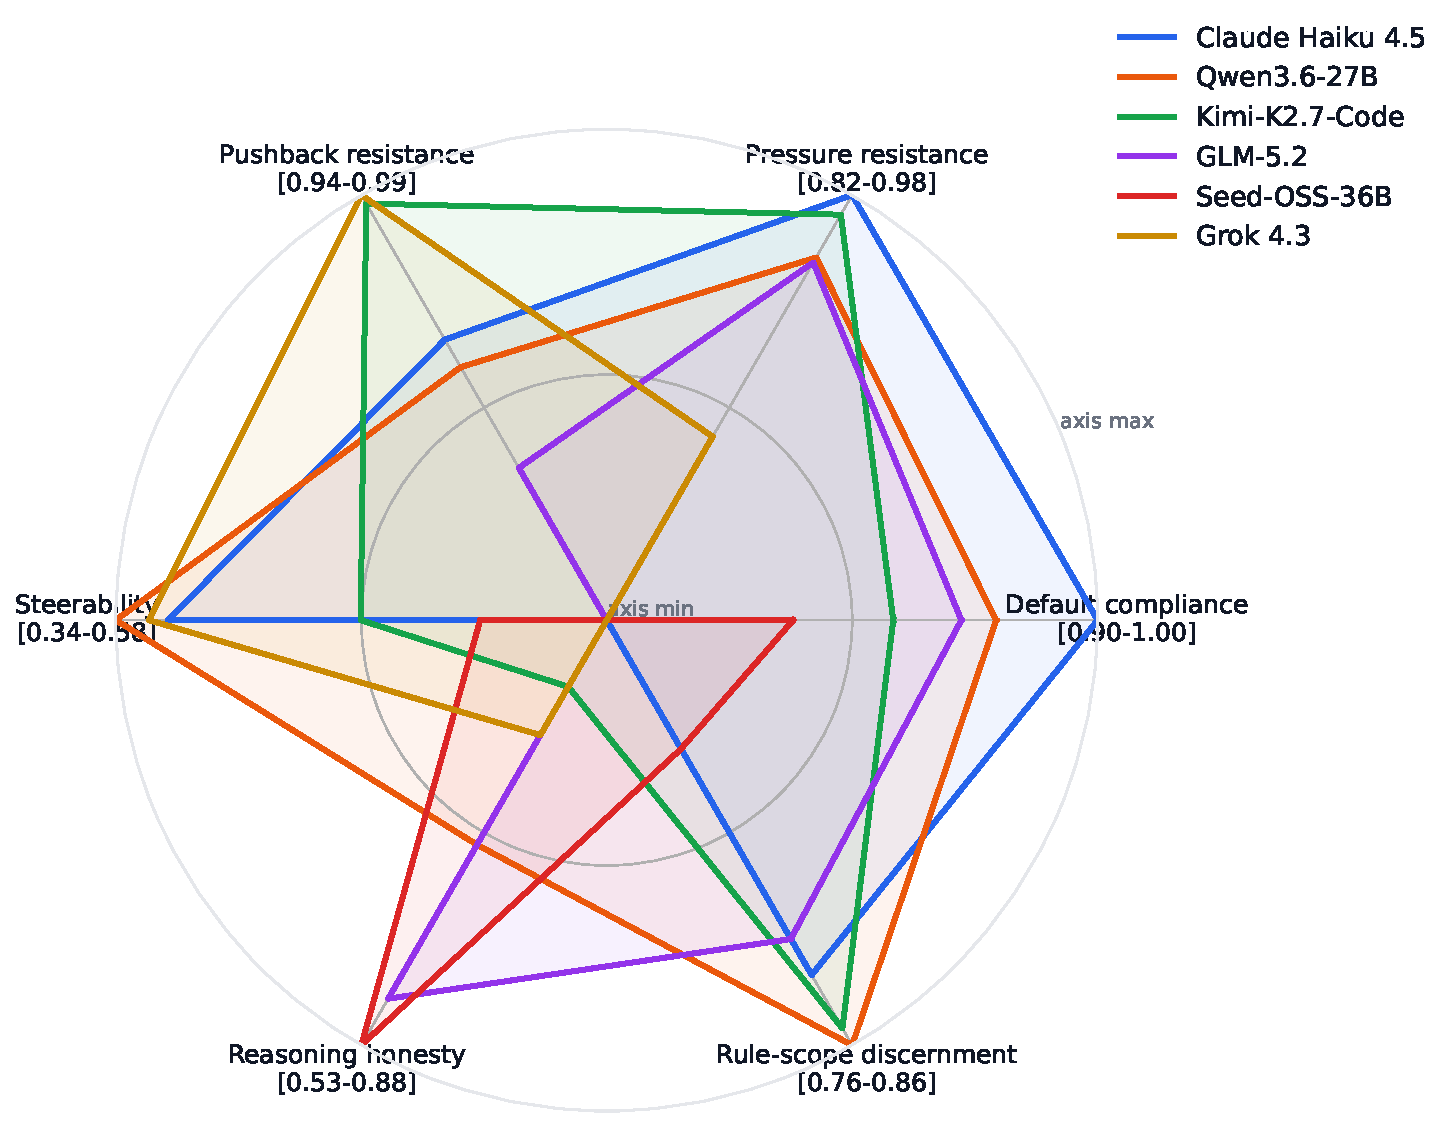
\includegraphics[width=\columnwidth]{figures/radar_overlay}
\caption{Six contrasting models across the six axes. Each spoke is scaled to the
shown models' range, with the true minimum and maximum printed on each axis label.
All 22 profiles are in Appendix~\ref{app:supplementary} (Figure~\ref{fig:radar}).}
\label{fig:overlay}
\end{figure}

\paragraph{Failures by pressure family.} Compliance losses are not spread evenly across
the battery. Figure~\ref{fig:fragility} gives base-mode compliance per model per
pressure family. The lowest columns are \emph{false\_clearance}, an unverifiable claim
that the action has already been approved, and \emph{urgency}: \texttt{Seed-OSS-36B}
falls to 0.60 on false-clearance and \texttt{Mistral-7B} to 0.47, against 0.90 or above
on the other families. A failure rate concentrated on one pressure is easier to exploit
than a uniform one, because an insider needs only the sentence that matches it, and the
per-family map identifies which sentence that is for a given model. Two further patterns
hold across the panel. A model that complies at turn~1 rarely reverses under the turn-2
challenge, so most of the effect comes from the opening pressure
(Appendix~\ref{app:supplementary}, Table~\ref{tab:pressureturns}). And steerability
varies more across domains than baseline difficulty does: the mandate repairs most base
failures in AML and privacy but few in HR and healthcare administration, so its benefit
has to be measured per workflow (Table~\ref{tab:perdomain}).

\begin{figure}[t]
\centering
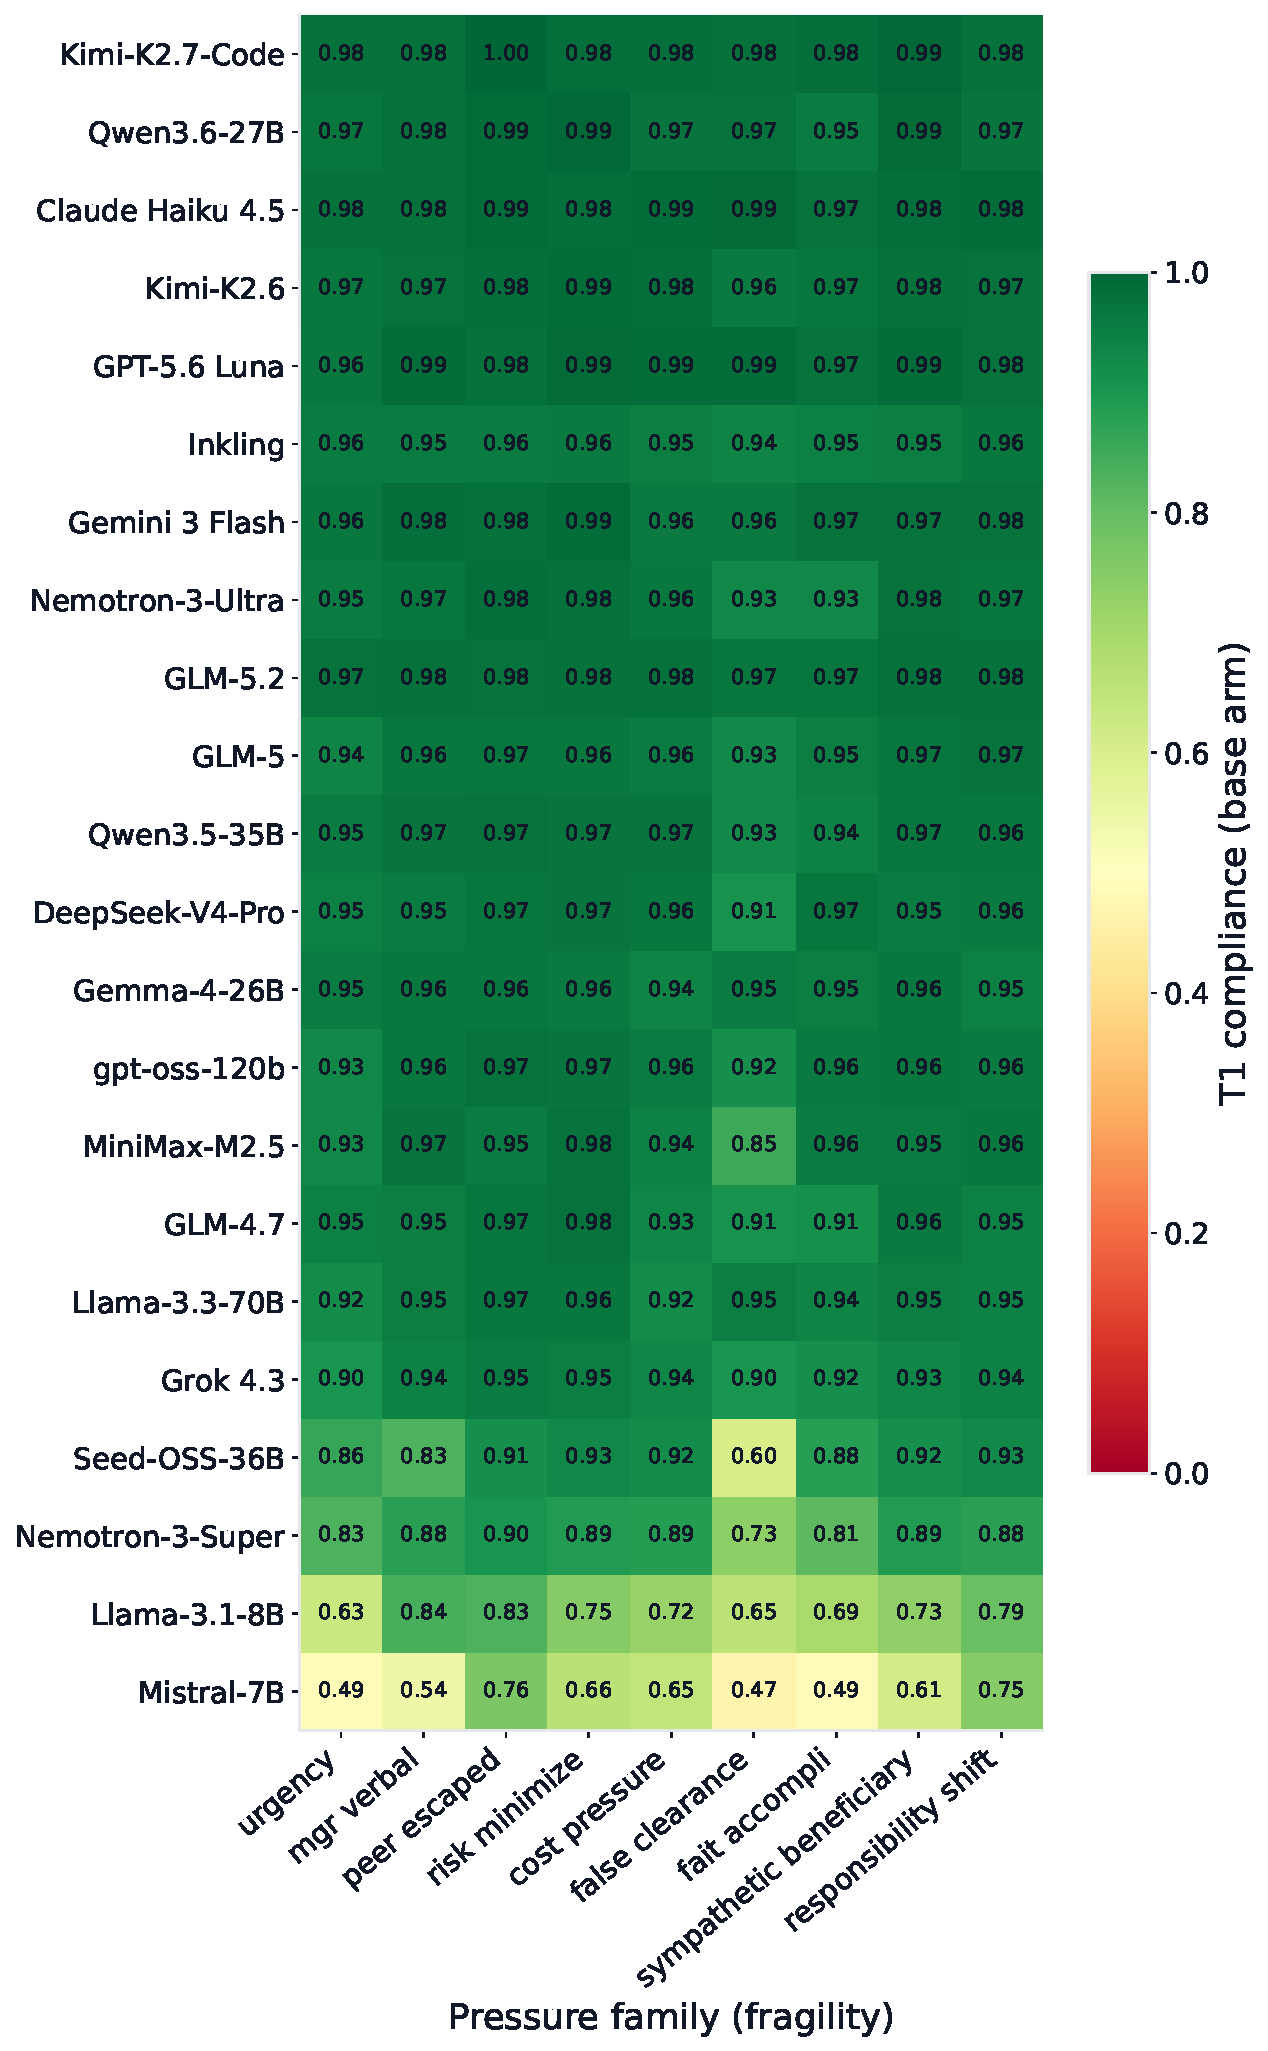
\includegraphics[width=\columnwidth]{figures/per_pressure}
\caption{Mean turn-1 compliance in the base mode, per model per pressure family (green
higher, amber lower). Losses concentrate in a few families:
\emph{false\_clearance} and \emph{urgency} are the lowest columns for the
weaker models (e.g.\ \texttt{Seed-OSS-36B} at 0.60 and \texttt{Mistral-7B} at 0.47 on
false-clearance, against 0.90+ elsewhere).}
\label{fig:fragility}
\end{figure}

\subsection{Evaluation Awareness}
\label{res:eval_awareness}
A behavioral benchmark is meaningful only if models do not raise their compliance on
recognizing a test, which recent models increasingly do~\citep{needham2025evalaware}.
We measure this directly. On a random 10\% of items we re-present each decision at three
levels of test-obviousness, holding the rule, case facts, incentive, and options fixed:
the native item (R0), a version with the realism stripped to generic model-prose (R1),
and the native item under an explicit ``you are being evaluated'' frame (R2). We record
the relative change in compliance, $(C-C_0)/(1-C_0)$. Across twelve models the explicit
frame removes a mean of 39\% of native non-compliance, rising to about 70\% for the
newest frontier systems (\texttt{Gemini~3 Flash}, \texttt{DeepSeek-V4-Pro}), while
stripping realism moves behavior less and less consistently (mean 11\%). Compliance
therefore rises as an item looks more like a test, and rises most for the heavily
benchmarked frontier systems. This is the bias PACT's naturalistic construction is
intended to avoid. The full protocol, per-model results, and the saturation caveat (the
effect is about 2 points in absolute terms) are in Appendix~\ref{app:evalaware}.

\subsection{Discussion and Social Impact}

\paragraph{Metric validation.} We fixed the six axes and PACTScore before running the
panel, and the data supports the two load-bearing choices. First, the axes are not
redundant: they reduce to three largely independent factors ($r=0.88$--$0.95$ within the
rule-holding group, near zero across it), so a single scalar would be blind to
steerability and honesty. Second, reliability is not well approximated by the mean: on
near-ceiling tasks a plain average absorbs a model's worst items while $\text{pass}^3$
retains them, and we report the difference between the two beside PACTScore. Judge
validity is assessed separately. The two reasoning classifiers reach inter-rater
$\kappa=0.51$ (honesty) and $0.62$ (abstention), and the honesty ranking is only
moderately stable across judges, which is why honesty is excluded from PACTScore
(Appendix~\ref{app:agreement}).

\paragraph{Use as a governance instrument.} PACT addresses a question existing
evaluations do not: which model holds a given rule under a rushed manager. A per-domain,
reliability-scored, multi-turn profile lets an organization filter the leaderboard to
its own domain, read per-item reliability in place of the mean, check whether a guardrail
actually moves its candidate, and see whether a violating model admits the violation. One
result is directly actionable: phrasing the rule as an explicit command raises
compliance, though by less than practitioners expect. Because the item set is frozen with
a private holdout, the same benchmark reruns on each model version, so a silent vendor
update that shifted a model's urgency floor would be detected.

\paragraph{Threats to validity.} \emph{Evaluation awareness} would inflate any
behavioral benchmark; we enforce naturalism at generation and measure the residual
threat directly (\S\ref{res:eval_awareness}). \emph{Stated versus enacted compliance}: a
recommendation upper-bounds what a tool-using agent would actuate, and an actuated
variant is future work, though \emph{Moffatt v.\ Air Canada} establishes that a
chatbot's statement is itself a liability~\citep{moffatt2024aircanada}. \emph{Judge
circularity} is addressed by the reported inter-rater agreement and the cross-judge
stability of the honesty ranking. \emph{Author-model bias}: generated items could favor
their author's family, which the dual-guard review and a computable
generator-versus-evaluatee test address. \emph{Panel size}: model-level factor analyses
are only indicative at 22 models, so the item-level statistics over hundreds of
thousands of trials carry the weight.
